\documentclass[border=4pt]{standalone}
\usepackage{amsmath,amssymb}
\usepackage{mathptmx} % Times-like serif to match IEEE
\usepackage{tikz}
\usetikzlibrary{arrows.meta,positioning,fit,calc}

\begin{document}
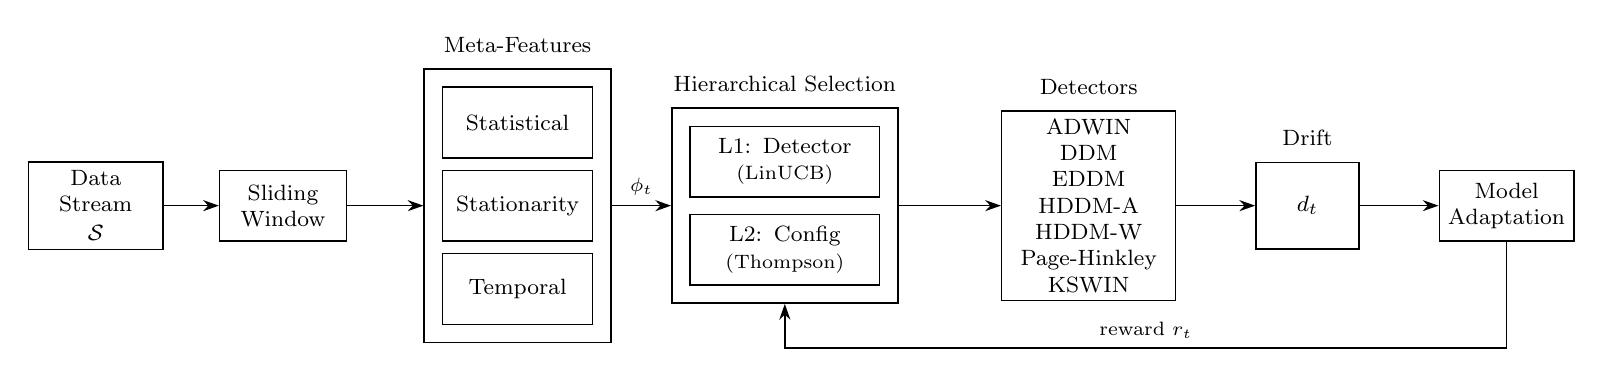
\begin{tikzpicture}[
  font=\footnotesize,
  >={Stealth[length=2mm,width=1.4mm]},
  box/.style={draw=black, line width=0.5pt, fill=white, align=center,
              inner sep=3pt, minimum height=9mm},
  grp/.style={draw=black, line width=0.6pt, fill=none, inner sep=2.2mm},
  ttl/.style={font=\footnotesize, align=center},
  to/.style={-{Stealth[length=2mm,width=1.4mm]}, line width=0.6pt},
]

% All stages centered on the y=0 line so every arrow runs straight.

% 1. Data Stream
\node[box, text width=15mm] (stream) {Data Stream\\[1pt]$\mathcal{S}$};

% 2. Sliding Window
\node[box, right=7mm of stream, text width=14mm] (win) {Sliding\\ Window};

% 3. Meta-Features  (anchor the MIDDLE sub-box to the line)
\node[box, right=12mm of win, text width=17mm] (mf2) {Stationarity};
\node[box, above=1.4mm of mf2, text width=17mm] (mf1) {Statistical};
\node[box, below=1.4mm of mf2, text width=17mm] (mf3) {Temporal};
\node[grp, fit=(mf1)(mf2)(mf3)] (meta) {};
\node[ttl, above=0.8mm of meta] {Meta-Features};

% 4. Hierarchical Selection  (anchor a midpoint on the line, boxes symmetric)
\coordinate[right=22mm of meta] (hc);
\node[box, above=1mm of hc, text width=22mm] (l1) {L1: Detector\\ \scriptsize(LinUCB)};
\node[box, below=1mm of hc, text width=22mm] (l2) {L2: Config\\ \scriptsize(Thompson)};
\node[grp, fit=(l1)(l2)] (hsel) {};
\node[ttl, above=0.8mm of hsel] {Hierarchical Selection};

% 5. Detector Portfolio
\node[box, right=13mm of hsel, text width=20mm] (port)
  {ADWIN\\ DDM\\ EDDM\\ HDDM-A\\ HDDM-W\\ Page-Hinkley\\ KSWIN};
\node[ttl, above=0.8mm of port] {Detectors};

% 6. Drift Signal
\node[box, right=10mm of port, text width=11mm, minimum height=11mm] (drift) {$d_t$};
\node[ttl, above=0.8mm of drift] {Drift};

% 7. Model Adaptation
\node[box, right=10mm of drift, text width=15mm] (adapt) {Model\\ Adaptation};

% forward arrows (all straight, common baseline)
\draw[to] (stream) -- (win);
\draw[to] (win) -- (meta);
\draw[to] (meta) -- node[above, font=\scriptsize]{$\phi_t$} (hsel);
\draw[to] (hsel) -- (port);
\draw[to] (port) -- (drift);
\draw[to] (drift) -- (adapt);

% feedback loop (routes below the tallest box, the portfolio)
\coordinate (lo) at ([yshift=-6mm]port.south);
\draw[to] (adapt.south) -- (adapt.south |- lo)
      -- node[above, font=\scriptsize]{reward $r_t$} (hsel.south |- lo)
      -- (hsel.south);

\end{tikzpicture}
\end{document}
